% This is included by the other .tex files.


\begin{frame}
    
\includegraphics[scale=.3]{images/logo-circl-Forensics.png}
    \begin{itemize}
        \item[]
        \item[]
        \item[] 15. Other Sources of Information
    \end{itemize}
\end{frame}


\begin{frame}[fragile]
  \frametitle{15.1 Recycle Bin}
    \begin{itemize}
        \item 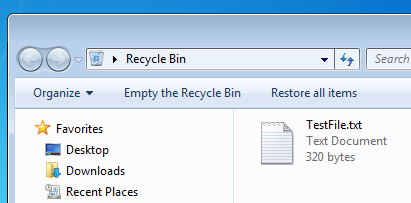
\includegraphics[scale=.18]{images/f15_recycle.png}
            \begin{itemize}
                \item 2019-04-30 17:31:57 UTC+2: Text file created
		\item 2019-04-30 17:34:44 UTC+2: Text file modified
		\item 2019-04-30 17:35:32 UTC+2: Text file deleted
		\item[]
            \end{itemize}
        \item Analyze Recycle.Bin:
  \begin{lstlisting}[basicstyle=\tiny]
/$Recycle.Bin/S-1-5-21-3408732720-2018246097-660081352-1000/
	129 Apr  5 11:46  desktop.ini
	544 Apr 30 17:35 '$IOMHI9A.txt'
	320 Apr 30 17:34 '$ROMHI9A.txt'

strings -el \$IOMHI9A.txt 
	C:\Users\John\Documents\recycleTest\TestFile.txt

strings \$ROMHI9A.txt 
		Test File
		=========
	This is a test file. It is just created to test Forensic
	Artifacts for the 'Recycle Bin'.
	.....
  \end{lstlisting}
    \end{itemize}
\end{frame}


\begin{frame}[fragile]
  \frametitle{15.1 Recycle Bin}
    \begin{itemize}
        \item Play Script:
            \begin{itemize}
                \item 2019-04-30 17:31:57 UTC+2: Text file created
		\item 2019-04-30 17:34:44 UTC+2: Text file modified
		\item 2019-04-30 17:35:32 UTC+2: Text file deleted
		\item[]
            \end{itemize}
        \item File system time line
    \end{itemize}
  \begin{lstlisting}[basicstyle=\tiny]
Fri Apr 05 2019 11:46:49
     328 m.c.      57-144-1 /$Recycle.Bin
     376 ...b    9632-144-1 /$Recycle.Bin/S-1-5-21- ..... -1000
     129 m.cb    9634-128-1 /$Recycle.Bin/S-1-5-21- ..... -1000/desktop.ini

Tue Apr 30 2019 17:31:57
     320 ...b   47164-128-1 /$Recycle.Bin/S-1-5-21- ..... -1000/$ROMHI9A.txt

Tue Apr 30 2019 17:34:44
     320 ma..   47164-128-1 /$Recycle.Bin/S-1-5-21- ..... -1000/$ROMHI9A.txt

Tue Apr 30 2019 17:35:32
     544 macb   44155-128-1 /$Recycle.Bin/S-1-5-21- ..... -1000/$IOMHI9A.txt
      48 mac.   47022-144-1 /Users/John/Documents/recycleTest
     320 ..c.   47164-128-1 /$Recycle.Bin/S-1-5-21- ..... -1000/$ROMHI9A.txt
     376 mac.    9632-144-1 /$Recycle.Bin/S-1-5-21- ..... -1000
  \end{lstlisting}
\end{frame}


\begin{frame}[fragile]
  \frametitle{15.2 LNK Files}
    \begin{itemize}
        \item Provide information about files accessed
        \begin{itemize}
            \item Local
            \item Network shares
            \item Appached devices
        \end{itemize}
    \end{itemize}
  \begin{lstlisting}[basicstyle=\tiny]
Thu May 02 2019 14:54:02
     280 ...b       43701-144-1 /Users/John/Documents/prefetchTest
  
Thu May 02 2019 14:54:28
      66 macb       43702-128-1 /Users/John/Documents/prefetchTest/
      				PreFetchTest.txt
    2779 macb       43716-128-4 /Users/John/AppData/Roaming/Microsoft/
    				Windows/Recent/PreFetchTest.txt.lnk
    1573 macb       43922-128-4 /Users/John/AppData/Roaming/Microsoft/
    				Windows/Recent/prefetchTest.lnk
  \end{lstlisting}
\end{frame}


\begin{frame}[fragile]
  \frametitle{15.2 LNK Files}
    \begin{itemize}
        \item Provide information about files accessed
        \begin{itemize}
            \item Local
            \item Network shares
            \item Appached devices
        \end{itemize}
    \end{itemize}
  \begin{lstlisting}[basicstyle=\tiny]
exiftool PreFetchTest.txt.lnk

	...
	Create Date         : 2019:05:02 14:54:28+02:00
	Access Date         : 2019:05:02 14:54:28+02:00
	Modify Date         : 2019:05:02 14:54:28+02:00
	Target File Size    : 66
	Icon Index          : (none)
	Run Window          : Normal
	Hot Key             : (none)
	Drive Type          : Fixed Disk
	Volume Label        :
	Local Base Path     : C:\Users\John\Documents\prefetchTest\
				PreFetchTest.txt
	...
  \end{lstlisting}
\end{frame}


\begin{frame}[fragile]
  \frametitle{15.3 XP Restore Points}
    \begin{itemize}
        \item Backups include:
        \begin{itemize}
	    \item Registry hives
            \item Local profiles
            \item ...
        \end{itemize}
        \item Created:
        \begin{itemize}
            \item Windwos XP: 24 hours
            \item Windows AutoUpdate
	    \item Installation of applications \& unsigned driver
            \item Restore opertion
            \item Manually
        \end{itemize}
        \item Provides:
        \begin{itemize}
	    \item \texttt{rp.log}
            \item Description of the cause
            \item Time stamp
            \item State of the system at different times
        \end{itemize}
    \end{itemize}
\end{frame}


\begin{frame}[fragile]
  \frametitle{15.4 Volume Shadow Copy}
    \begin{itemize}
	    \item On Windows: \texttt{C:/>vssadmin list shadows /for=c:/}
	    \item Infected PC:
  \end{itemize}
  \begin{lstlisting}[basicstyle=\tiny]
vshadowinfo -o $((512*206848)) 8d34ce.raw 

    Volume Shadow Snapshot information:
	Number of stores:	1

    Store: 1
	Identifier		: 237c8de3-5b99-11e9-9925-080027062798
	Shadow copy set ID	: 33eb3a7b-6d03-4045-aa70-37b714d49c72
	Creation time		: Apr 10, 2019 14:06:30.365699200 UTC
	Shadow copy ID		: 34d9910b-ac1d-4b10-b282-89dde217d0fb
	Volume size		: 11 GiB (12777947136 bytes)
	Attribute flags		: 0x0042000d

sudo vshadowmount -o $((512*206848)) 8d34ce.raw /mount/vss/

sudo ls -l /mount/vss/
	-r--r--r-- 1 root root 12777947136 Jan  1  1970 vss1

sudo file /mount/vss/vss1
	/mount/vss/vss1: DOS/MBR boot sector, code offset 0x52+2, OEM-ID "NTFS 

sudo mount -o ro /mount/vss/vss1 /mnt/
  \end{lstlisting}
\end{frame}


\begin{frame}[fragile]
  \frametitle{15.5 Prefetch Files \& SuperFetch}
    \begin{itemize}
        \item Improve performance
        \item Boot prefetching
	\item Application prefetching
	\item Collect information about all files accessed
	\item Take all resources as one file
	\item Resources are not spread arround the disk
	\item Wait 10sec after application started
	\item[] $\to$ Better performance
	\item[] $\to$ Example: 
    \end{itemize}
  \begin{lstlisting}[basicstyle=\tiny]
Thu May 02 2019 14:52:40
    179712 .a..      10940-128-3 /Windows/System32/notepad.exe
    179712 .a..      10940-128-3 /Windows/notepad.exe

Thu May 02 2019 14:52:50
        56 mac.      42729-144-6 /Windows/Prefetch
     16280 macb      43700-128-4 /Windows/Prefetch/NOTEPAD.EXE-D8414F97.pf
  \end{lstlisting}
\end{frame}


\begin{frame}[fragile]
  \frametitle{15.5 Prefetch Files \& SuperFetch}
    \begin{itemize}
        \item Information found:
        \begin{itemize}
            \item Application launched number of times
            \item Application launched last time
            \item Path to application
            \item Path to other resources
        \end{itemize}
        \item Indirect benefits:
        \begin{itemize}
            \item Which user was logged in run the application
            \item Deleted applications run once in time
        \end{itemize}
    \end{itemize}
  \begin{lstlisting}[basicstyle=\tiny]
prefetch.py -f NOTEPAD.EXE-D8414F97.pf

	Executable Name: NOTEPAD.EXE
	Run count: 1
	Last Executed: 2019-05-02 12:52:40.339584

	Resources loaded:
	1:    \DEVICE\HARDDISKVOLUME2\WINDOWS\SYSTEM32\NTDLL.DLL
	2:    \DEVICE\HARDDISKVOLUME2\WINDOWS\SYSTEM32\KERNEL32.DLL
	3:    \DEVICE\HARDDISKVOLUME2\WINDOWS\SYSTEM32\APISETSCHEMA.DLL
	4:    \DEVICE\HARDDISKVOLUME2\WINDOWS\SYSTEM32\KERNELBASE.DLL
	.....
  \end{lstlisting}
\end{frame}




